\subsection{Comparison with $\BKZ$} \label{subsec:ComparisonWithBKZ}

In this section we compare the constants in the exponents of the running time of algorithms for $\appSVP$ on the $2n$-dimensional lattice $\qLATTp(\AMat)$. The length of the target vector is $\|\vvec \| \leq n^{\cg} \det(\qLATTp(\AMat))^{1/(2n)}$. The algorithms in consideration are the $\BKZ$ lattice-reduction algorithm with a block-size $\beta = \TLandau(n)$ and our two algorithms Alg.~\ref{alg:ApproxSVP} and Alg.~\ref{alg:ApproxSVPImprived}. For the \BKZ algorithm, we have the following simple lemma.

\begin{lemma} 
	Given on input (1) a $2n$-dimensional $q$-ary lattice $\qLATTp(\AMat)$ with a basis as in Eq.~(\ref{eq:BasisD}), and (2) an approximation factor $\gamma = \bigO(n^{\cg})$, the \BKZ basis-reduction algorithm instantiated with an \SVP oracle that runs in time $\bigO(2^{(\cBKZ + \smallo(1))n})$, outputs a vector of desired length in time
	\[
		T(\BKZ) = 2^{\Big( \tfrac{\cBKZ }{\cg+1/2} + \smallo(1) \Big) n}.
	\]
\end{lemma}
\begin{proof}
	The result follows immediately from Eq.~(\ref{eq:b1norm_ineq}): solving for $\beta$ the inequality $\beta^{\tfrac{2n}{2\beta}} \cdot \det (\qLATTp(\AMat))^{\tfrac{1}{2n}} \leq n^{\cg+1/2} \cdot \det (\qLATTp(\AMat))^{1/(2n)}$, yields $\beta = \Big( \frac{\cBKZ}{\cg+1/2} + \smallo(1) \Big)n$.
\end{proof}

One should not be surprised that the constant for $\BKZ$ does not depend on $\cq$: the size of the modulus only affects polynomial pre-factors in the complexity of the algorithm \cite{C:HanPujSte11}.

As discussed in Chap.~\ref{chap:Prelim} and Chap.~\ref{chap:LWEasBDD}, we can instantiate an \SVP oracle using provable algorithms with $\cBKZ = 1$, or using algorithms that rely on some heuristics with $\cBKZ = 0.292$. These together with our results on combinatorial algorithms for $\appSVP$ given in Thms.~\ref{thm:appSVP} and \ref{thm:appSVPImproved}, allow us to compare all four algorithms and deduce which one performs best for given $\cq, \cg$. 

%
% Figures
%

\definecolor{Crimson}{RGB}{220,20,60}
\definecolor{Turquoise}{RGB}{64, 224, 208}
\definecolor{LightSalmon}{RGB}{255, 160, 122}
\definecolor{DarkOliveGreen}{RGB}{85,107,47}

\definecolor{Orange}{RGB}{255, 165,0}

\begin{figure}[h]
	\centering
	\begin{subfigure}[t]{0.49\textwidth}
		\centering
		\begin{tikzpicture}
		\node[anchor=south west,inner sep=0] (image) at (0,0) {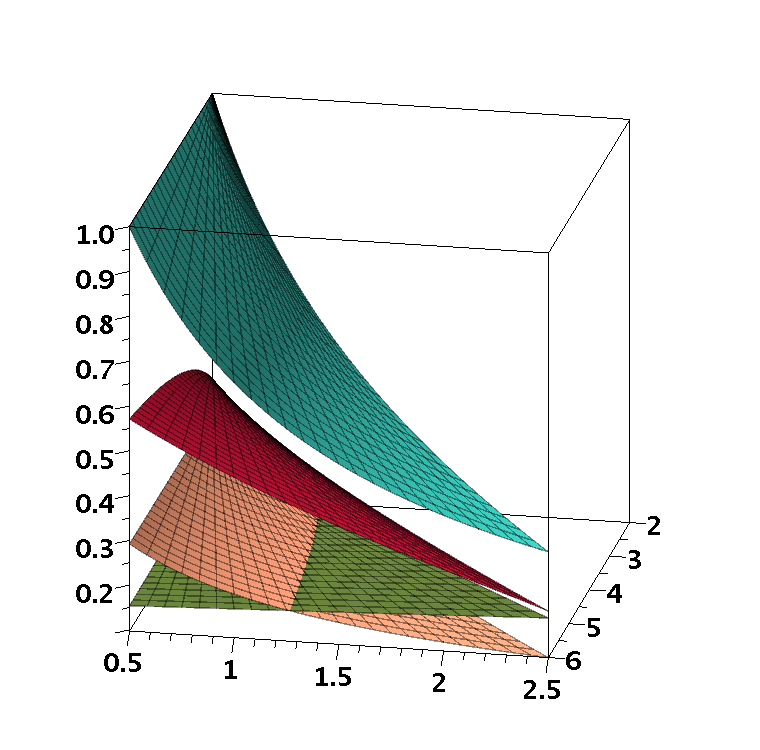
\includegraphics[width=0.95\textwidth, trim={10mm 10mm 10mm 10mm}]{Plots/Plot3dQary}};
		
		\node[draw=none] at (6.5, 1.0) {$\cq$};
		\node[draw=none] at (3.0, 0.05) {$\cg$};
		\node[draw=none] at (.2, 3.05) {$\const$};
		
		\draw[fill=Turquoise, opacity=0.9] (1.2, -0.3) rectangle (1.5, 0.0) node[yshift=-5pt, xshift=14pt]{\scriptsize $\cBKZ=1$};
		
		\draw[fill=Crimson, opacity=0.9] (3.2, -0.3) rectangle (3.5, 0.0) node[yshift=-5pt, xshift=14pt]{\scriptsize Alg.~\ref{alg:ApproxSVP}};
		
		\draw[fill=LightSalmon, opacity=0.9] (1.2, -0.8) rectangle (1.5, -0.5) node[yshift=-5pt, xshift=21pt]{\scriptsize $\cBKZ=0.292$};
		
		\draw[fill=DarkOliveGreen, opacity=0.9] (3.2, -0.8) rectangle (3.5, -0.5) node[yshift=-5pt, xshift=14pt]{\scriptsize Alg.~\ref{alg:ApproxSVPImprived}};
		
		\end{tikzpicture}
	\end{subfigure}
	\begin{subfigure}[t]{0.45\textwidth}
		\centering
		\begin{tikzpicture}
		\node[anchor=south west,inner sep=0] (image) at (0,0) {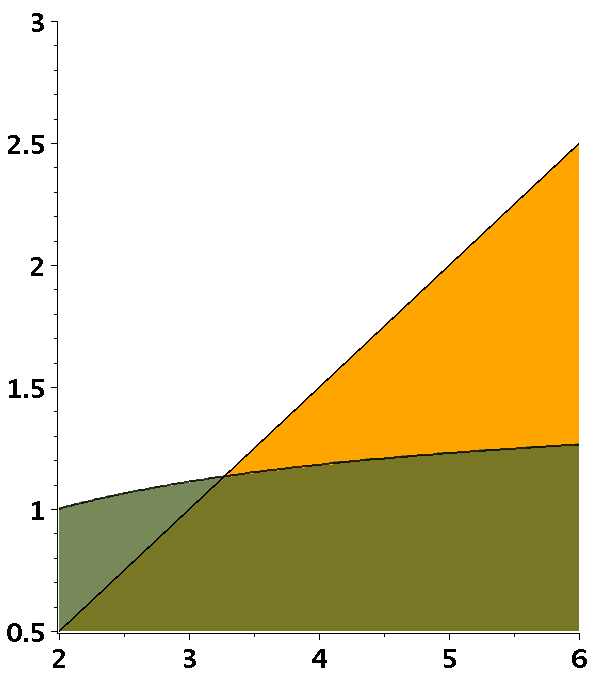
\includegraphics[width=0.80\textwidth, trim={0 0 0 13cm}]{Plots/PlotQAryIneq}};
		
		\node[draw=none] at (-0.01, 3.3) {$\cg$};
		\node[draw=none] at (3.0, -0.1) {$\cq$};
		
		\draw[fill=Orange, opacity=0.9] (0.3, -0.6) rectangle (0.6, -0.3) node[yshift=-5pt, xshift=25pt]{\scriptsize $\cg< \tfrac{\cq}{2} - \tfrac{1}{2}$};
		
		\draw[fill=DarkOliveGreen, opacity=0.9] (2.8, -0.6) rectangle (3.1, -0.3) node[yshift=-5pt, xshift=38pt]{\scriptsize Alg.~\ref{alg:ApproxSVP} $\leq \cBKZ \mkern-3mu=0.292$};
		
		\end{tikzpicture}
	\end{subfigure}
	\caption[Comparison of algorithms for $\appSVP$]{Comparison of two families algorithms for $\appSVP$: those that are based on \BKZ reduction and combinatorial ones. The considered parameter range  is $\cq=[2, \ldots, 6], \cg=[0.5, \ldots \cq/2 - 1/2]$.}
	\label{fig:appSVPCompare}
\end{figure}

\paragraph{Combinatorial \DUAL attack on \LWE.} Recall the \DUAL attack on \LWE with parameters $n, q = \bigO(n^{\cq})$, $\alpha =~ \bigO(n^{-\ca})$ (see Alg.~\ref{alg:Dual} in Sect.~\ref{sec:OtherAttacks}). As the main subroutine, it runs an $\appSVP$ solver on the lattice $\qLATTp(\AMat)$. The approximation factor $\gamma$ depends on the number of \LWE samples provided. Instead of running a $\beta$-\BKZ reduction to solve $\appSVP$ as we do in Sect.~\ref{sec:OtherAttacks}, we can run a combinatorial algorithm for the search of a short vector in $\qLATTp(\AMat)$. In case, we have exponentially-many samples, we run our Alg.~\ref{alg:ApproxSVP} with $\cg = \ca-\cq/2$ in which case the running time of the (combinatorial) \DUAL attack on $\LWE$ is $2^{(\const+\smallo(1))n}$ where $\const = \big(2 \ln\big(\tfrac{\cq}{\cq-\ca} \big) \big)^{-1}$. In case $m=\TLandau(n \log n)$, we resort to the sample amplification which decreases $\ca$ by $1/2$. This results in a smaller approximation factor leading to a worse running time constant $\const = \big(2 \ln\big(\tfrac{\cq}{\cq-\ca+1/2} \big) \big)^{-1}$.